\chapter{Introduction}

- deepfake is buzzword (no agreed-upon technical definition)
- ...

\chapter{Deepfakes}

The creation of fake media and their detection have been a problem since photography was invented. Digital photography or video with tools such as GIMP, Adobe Photoshop or Adobe After Effects allows more people to create fakes than before, still some experience in this area is needed. Media that have been modified or otherwise manipulated are called synthetic media, and they do not depend on whether it is an analogue or digital medium. Deepfakes also fall under this category \cite{IncreasingThreatofDeepfakeIdentites}. Tools powered by deep learning allow unexperienced users to easily create trusted fakes. 

The quality of deepfakes reached a level when a trained person or even an experienced researcher in this field has a problem of spotting them. This fast development allows creating realistically looking assets to art photography or movie production, unfortunately, it can be used for malicious purposes like creating fake porn videos to blackmail people or manipulate public via fake news. There are many use cases where deepfakes can be applied.

It is putting huge pressure on researchers to develop new forensics tools or any technology which will prevent malicious usage of deepfakes. As mentioned before, creating fakes is not new, and a whole field of study engaged in spotting fakes and developing techniques over 15 years. Despite continuous research efforts in the past, the advent of deep learning changed the rules of the game. \cite{MediaForensicsandDeepFakes}

\section{Human capabilities of deepfake detection}

The human ability to recognize fake materials from the originals is in contradiction to their quality. Korshunov and Marcel confirmed this in their research. They created a questionnaire containing several videos, and the subject (interviewee) had to answer after watching the video whether the person in the video was genuine, fake, or they are uncertain. The videos were manually divided into five categories (very easy, easy, moderate, difficult, and very difficult, original). 

Videos were split into several categories manually by researchers probably without usage of any metrics but based on their personal feelings, and ANOVA test shows there is an overlap in several categories, so several videos could be moved to different category. However, the categories are still significantly different. 

The results of test in Fig. \ref{fig:subjective_answers} certainly demonstrate that people's recognition ability decreases significantly as the quality of deepfakes increases. Also, the audience of this test knows they are looking for fakes, otherwise we can expect worse results if there will be unsuspected audience (for example: deepfakes on social media). It is quite alarming that the correct answers in the category of “very easy” reach only 71,1 \%. The quality of deepfake increases over time, thus it can be expected that human recognition ability will continue to decrease. \cite{TheThreatOfDeepfakes}

\begin{figure}[H]
    \begin{subfigure}[h]{.45\linewidth}
        \centering
        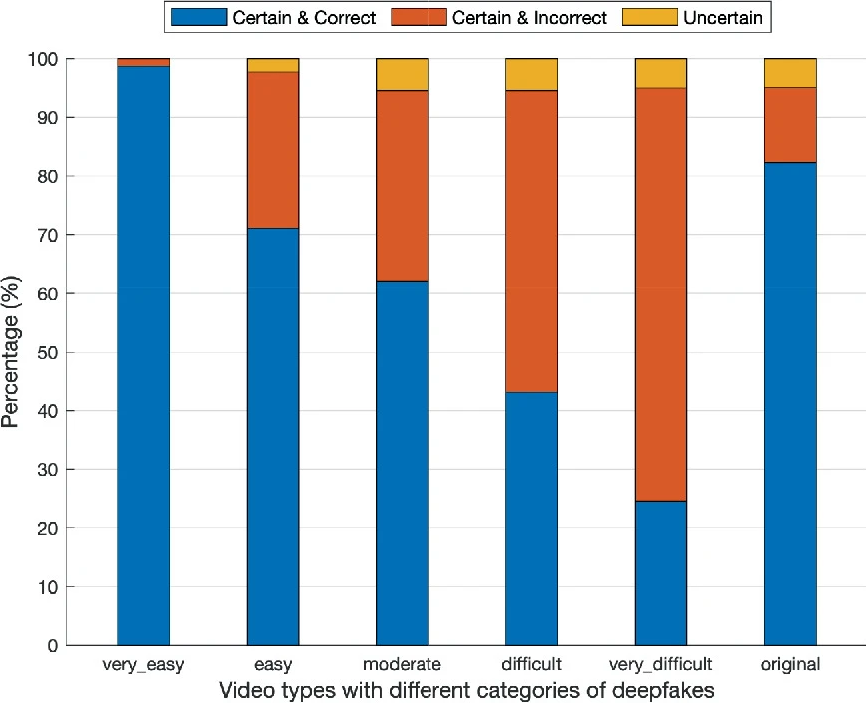
\includegraphics[width=1\linewidth]{other-fig/subjective_answers_a.png}
        \caption{Subjective answers}
    \end{subfigure}
    \hfill
    \begin{subfigure}[h]{.45\linewidth}
        \centering
        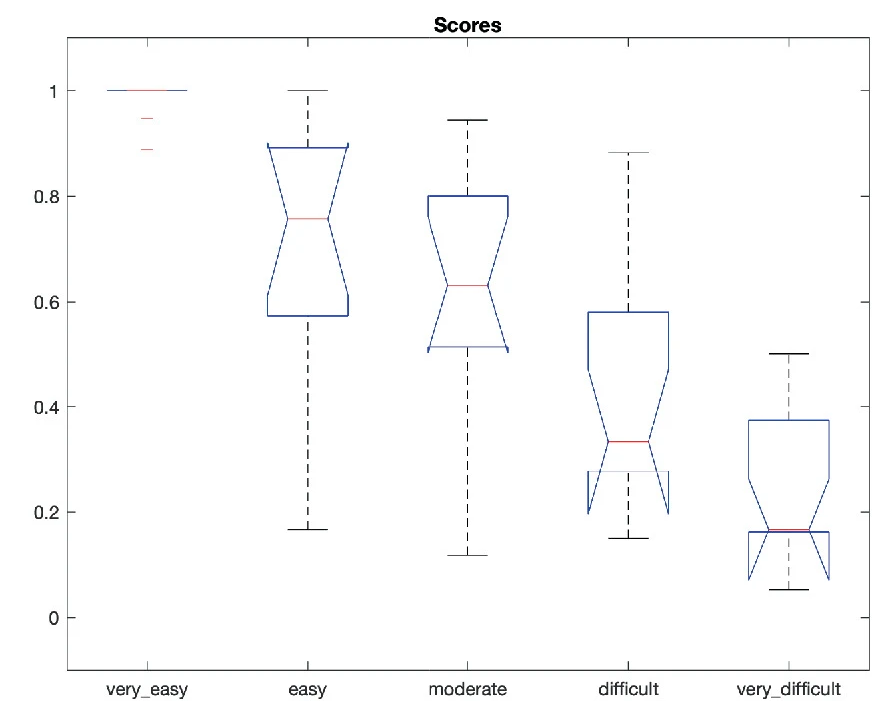
\includegraphics[width=1\linewidth]{other-fig/subjective_answers_b.png}
        \caption{ANOVA test}
    \end{subfigure}
    \caption{Subjective answers and median values with error bars from ANOVA test for different deepfakehttps://www.overleaf.com/project/6373f30660c2425f4720defb categories. Retrieved from \cite{TheThreatOfDeepfakes}.}
    \label{fig:subjective_answers}
\end{figure}

Another research tested only recognition of audio tracks and they were comparing humans versus computer programmes. Attendees had a correct classification between fakes and origins 67 \% after the first several rounds. Their accuracy increased while listening and answering to more tracks, but the value stabilizes to 80 \%. On average, trained AI performs about 10 \% better than human, but this result highly depends on difference of learning and test dataset. Still, it shows that the computer can outperform humans in spotting deepfakes. \cite{HumanPerceptionAudio}

\section{Potentional risks}

Humans are not good at recognizing deepfakes, but “why should we be worried?”. Almost every technology humankind created could be used for good or bad – deepfake is no exception. There are plenty different deepfake categories, and each has its own attack vector or use case. This section is describing potential risks of those categories and their closer description will be covered in next section \ref{section:deepfakes_creation}.

Deepfakes are about gaining someone’s trust or influence him. For the last couple of years there has been an increasing trend to scam people, mostly via phone or computer. Targeting only one person/victim, for example, to gain their money or information. Those attacks are getting better and more credible and using deepfake to impersonate close friend of victim could be next step how to improve it, if it is not already happening. \cite{HybridVishingAttacksSkyrocketing}

Creating “fake news” to influence a large audience is the most common use case of deepfakes because we live in an information era. There are many targets of “fake news” such as rigging elections, demoralizing military units, or manipulating the stock market. In this case, politicians, celebrities, and significant personalities will be used in deepfakes to influence audience. We can only imagine what one person or high quality deepfake can change with enough media reach. For example, after one tweet from Elon Musk about Tesla’s stock, sends shares down more than 10 \% almost immediately \cite{ElonMusksTweets}. \cite{IncreasingThreatofDeepfakeIdentites}

A real example of deepfake is famous video with Barak Obama insulting Donald Trump, which should spread awareness regarding the fast developing category of new threads \footnote{https://www.buzzfeed.com/craigsilverman/obama-jordan-peele-deepfake-video-debunk-buzzfeed}. Several years later another video stating Volodimir Zelenskyj talking about surrendering, it was proved that it is a manipulated video, and its purpose was to demoralize Ukraine army and make them capitulate \footnote{https://www.youtube.com/watch?v=X17yrEV5sl4}.

Another field where deepfakes could be used is to tricky biometrics systems in which the attacker is a different person to the gain access to the building, to secured equipment, etc. It was proven that biometrics system is not ready to deal with deepfakes, and it will probably require to add a new module to authentication pipeline which will be detecting deepfakes. Face or voice biometrics recognition systems are in greatest danger. The falsification of documents is related to this topic and there was a case of smuggling people across borders with an official passport containing morphed photos of two individuals.
% TODO: [DawnOfTextDependentSociety], [DigitalFaceManipulation], [MorphingAttackPotential]

These cases are only the tip of the iceberg, and in the future, everyone should ask if video on social media with film celebrity is real or even worse, if the evidence in courts is trustworthy or not. The solution for this will be easy to use tools capable of detecting deepfakes for unskilled users and also for experts.

\section{Types of deepfakes and their creation process}
\label{section:deepfakes_creation}

There are plenty of methods on how to create deepfakes, and as its name suggests some of them are based on deep neural networks, but not exclusively.  This section describes most common types of learning networks used for creating image/video or voice deepfakes. One of the most popular types for face deepfakes is Generative adversarial network (GAN), and it is used to create completely new faces or face manipulations.

Each method leaves traces in the medium that can then be detected. This is one way to recognize deepfakes so understanding process of creation is an advantage. Detecting will be described in more detail in Chapter \ref{chapter:deepfake_detectoin}.

\subsection{Neural networks}

All the facts regarding neural networks were retrieved from \cite{CreationandDetectionofDeepfakes}. Neural networks are composited from neurons arranged in layers, and each layer is connected sequentially via synapses. Synapses are weighed, and the process of finding the proper value of all weights is called a learning neural network. To obtain results from the input of n-dimensional “x” process “forward-propagation” is used to propagate “x” through each layer.

Input to layer is vector “a” of values calculated by previous layer or in case of first layer “x” itself. That means result of each layer is also vector calculated by activation function f(a*W+b), where f is activation function (Sigmod, ReLU, etc.), “a” is input vector, W is matrix of weights between layers i and i+1 and b is dimensional bias. Dimensional bias is a constant offset that helps the network shift the activation function toward the positive or negative side \cite{NeuralNetworkBias}.

Now let’s consider the neural network M as a black box and denote its execution as M(x) = y. Supervise learning to train M is using paired samples with from (xi, yi) and loss function L is defined. Loss function is to generate a signal at the output of M and propagate him back to find error of each weight in synapses.

Optimalization algorithms such as gradient descent are then used to calculate new weights of M for the number of epochs. As a result of this process, the network learns the function M(xi) ~~ yi and is capable of making prediction on unseen data. More detailed descriptions of this could be found in the work of Y. Mirsky and W. Lee \cite{CreationandDetectionofDeepfakes}.

Next list shows types of neural networks used for generating deepfakes \cite{CreationandDetectionofDeepfakes}:

\begin{itemize}
\item Generative Adversarial Networks (GAN) – Consist of two neural networks working against each other. One layer is generator and second is discriminator. Generator producing fake features trying to fool discriminator, on the other hand, discriminator is learning to distinguish between real sample and fake one.
\item Encoder-Decoder networks (ED) – Contains at least two networks, encoder and decoder. It has narrowed layers towards its center. If encoder “En” and decoder “De” are symmetric and they are trained as De(En(x)) = x, then the network is called autoencoder. Generating deepfakes using ED trained with function De(En(x)) = xg, where xg is fake generated features. There is possibility to use multiple different ED chained after each other or using specific variant of ED called variational autoencoder.
\item Convolutional Neural Network (CNN) – CNN is learning pattern hierarchies in the data. For deepfakes purposes, it learns filters applied over the input and forming an abstract feature map as the output.
\item Recurrent Neural Networks (RNN) – RNN can handle variable length data and it is remembering stat after processing which can be used in next iteration. RNN are mostly used in audio.
\end{itemize}

Each category has its own subcategories that have small modifications or using some techniques from different category. 

\subsection{Voice deepfakes}

Speech synthesis is divided into two categories based on input data. Text to speech (TTS) converts written text to artificial speech and second category is called voice conversion (VC). The voice conversion consumes source voice, and both methods produce synthesis voice saying desired phrases specified by the input. \cite{ApplicabilityOfDeepfakes}

Voice deepfakes are used independently or with deepfake video (full puppet). Creating synthesis voice is computationally challenging and one of the goals is making real-time voice conversion. There are several projects that are trying to accomplish this \footnote{https://github.com/SolomidHero/real-time-voice-conversion} \footnote{https://www.resemble.ai/speech-to-speech/}.

\subsection{Image or video deepfakes}

The list of the following deepfakes is based on the work R. Tolosana, et al. \cite{IntroductionToDigitalFaceManipulation}:

\begin{itemize}
\item Identity swap – Replacing the face of subject with the face of target as shown in Fig. \ref{fig:idenity_swap}. There are two different approaches, classical computer graphics-based technique and deep learning technique. Generally, the process of swap could be described as face detection, cropping, extraction of intermediate representations, synthesis of new face, and blending the generated face.
\begin{figure}[H]
    \centering
    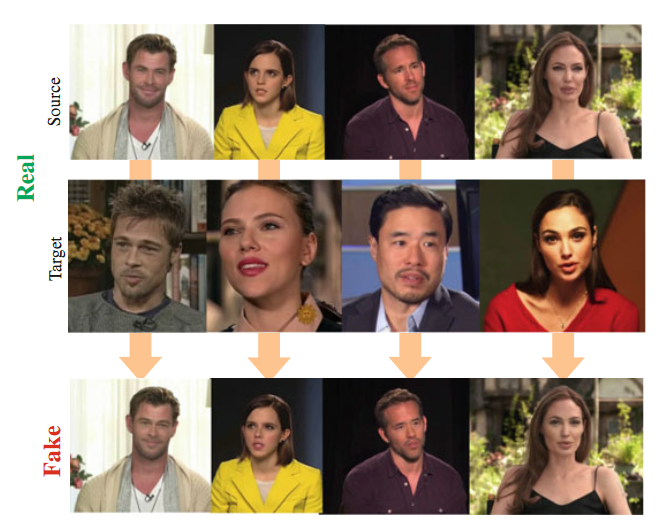
\includegraphics[width=.68\linewidth]{other-fig/idenity_swap.png}        
    \caption{XXX. Retrieved from \cite{IntroductionToDigitalFaceManipulation}.}
\label{fig:idenity_swap}
\end{figure}

\item Full puppet – Method related to identity swap allows creation of so-called puppet. One person (master) is source of facial expression and body movements that are mapped onto target person as shown in Fig. \ref{fig:full_puppet}. \cite{IncreasingThreatofDeepfakeIdentites}
\begin{figure}[H]
    \centering
    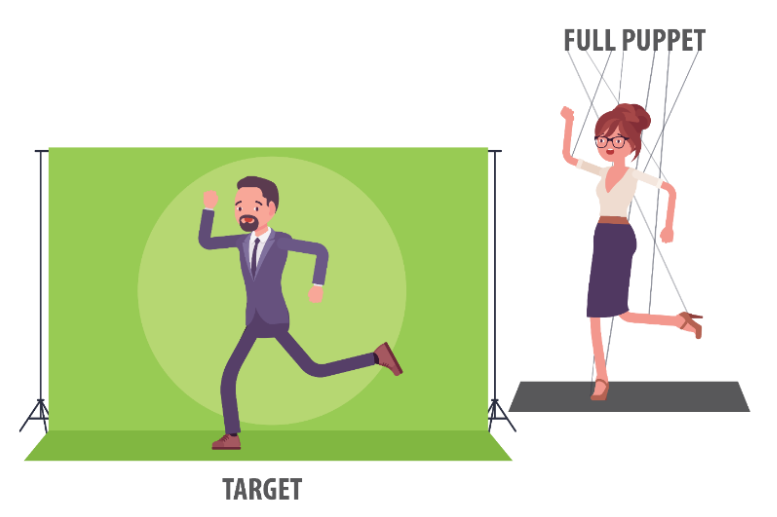
\includegraphics[width=.6\linewidth]{other-fig/full_puppet.png}        
    \caption{XXX. Retrieved from \cite{TheThreatOfDeepfakes}.}
\label{fig:full_puppet}
\end{figure}

\item Morphing – It is a type of manipulation that is used to create artificial biometric face samples. Final face contains resemble biometric information of two or more individuals. It should be possible to be successfully verified by biometrics systems for all individuals who were source for given deepfake. Fig. \ref{fig:morphing} shows an example of a morphed image.
\begin{figure}[H]
    \centering
    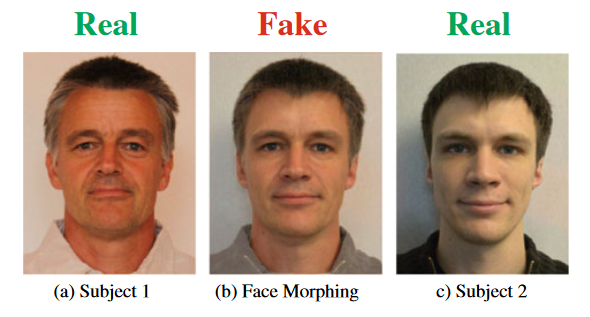
\includegraphics[width=.5\linewidth]{other-fig/morphing.png}        
    \caption{XXX. Retrieved from \cite{IntroductionToDigitalFaceManipulation}.}
\label{fig:morphing}
\end{figure}

\item Attribute manipulation – Face editing or face retouching technique involves modifying some attributes such as length or color of hair, color of skin, sex, age, adding glasses or other artefacts, and more. Fig. \ref{fig:attribute_manipulation} shows an example of this technique.
\begin{figure}[H]
    \centering
    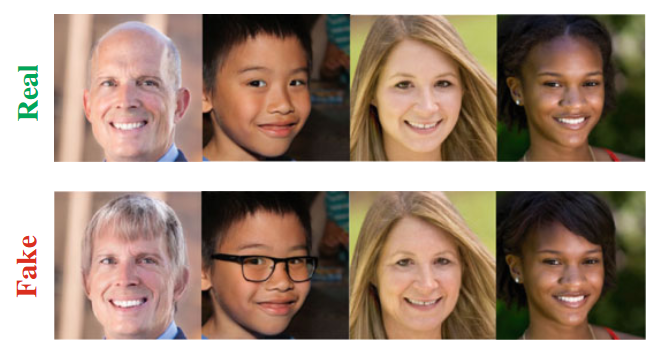
\includegraphics[width=.6\linewidth]{other-fig/attribute_manipulation.png}        
    \caption{XXX. Retrieved from \cite{IntroductionToDigitalFaceManipulation}.}
\label{fig:attribute_manipulation}
\end{figure}

\item Expression swap – Modifying facial expression of the subject as shown in Fig. \ref{fig:expression_swap}. This technique is used as one of part for full puppet.
\begin{figure}[H]
    \centering
    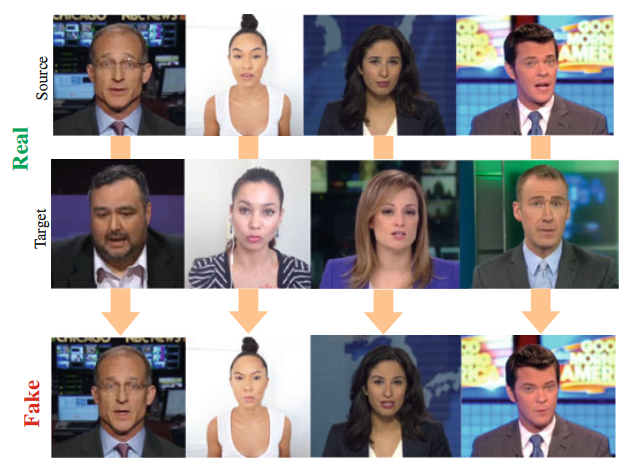
\includegraphics[width=.64\linewidth]{other-fig/expression_swap.png}        
    \caption{XXX. Retrieved from \cite{IntroductionToDigitalFaceManipulation}.}
\label{fig:expression_swap}
\end{figure}

\item Audio/text to video – This method related to expression swap synthesising facial expression from audio or text. It is also known as lip-sync deepfakes. Diagram in Fig. \ref{fig:audio_to_video} shows how this method works.
\begin{figure}[H]
    \centering
    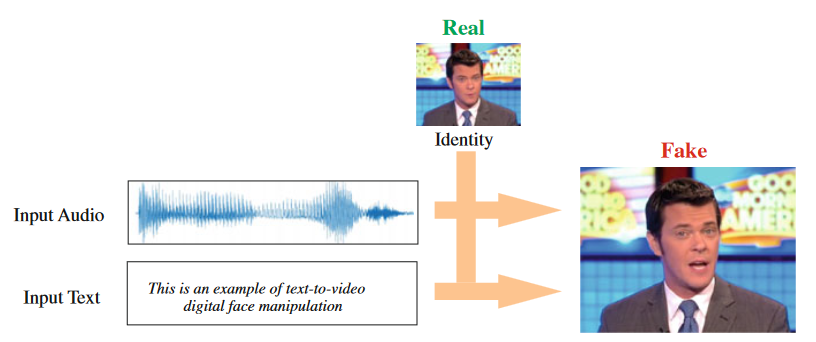
\includegraphics[width=.65\linewidth]{other-fig/audio_to_video.png}        
    \caption{XXX. Retrieved from \cite{IntroductionToDigitalFaceManipulation}.}
\label{fig:audio_to_video}
\end{figure}
\end{itemize}

Creating deepfakes nowadays is complex task and many deepfakes is using more techniques so that they could be included into more than one category. Attackers could create deepfake that will fall under identity swap category and after that use attribute manipulation to tune final results.

\chapter{Deepfake detection}
\label{chapter:deepfake_detectoin}

\chapter{Analysis of existing tools for detecting deepfakes}
\section{Deepware}
    - https://scanner.deepware.ai/developer/
\section{Deepstar}
    - https://www.zerofox.com/deepstar-open-source-toolkit/


\chapter{Architecture and technologies analysis}
\section{Requirements}
\section{Containerazation}
\section{Web server}
\section{Web browser plugin}
\section{Selected detection methods}

\chapter{Framework architecture}
\section{High level architecture}
\section{Containerazation and scaling}
\section{Input layer}
\section{Data preparation layer}
\section{Inividual detection containers}

\chapter{Client architecture}
\section{Web browser plugin}

\chapter{Framework implementation}

\chapter{Client implementation}

\chapter{Test experiment and results}

\chapter{Conclusion}